\chapter{ANÁLISE DE DADOS DO SISTEMA PACIFICADOR WEB}
% \hspace{1.5cm}
A construção de um modelo capaz de quantificar a utilização do Sistema de Comando e Controle nos Comandos Militares, foi a realização de um estudo estatístico sobre as variáveis: centro de operação; agente; incidente; ação; e ponto de interesse, colhidas na base de dados do sistema referente ao período de jan/2017 à out/2019, dos eventos e operações que aconteceram nestes período. Nesta análise exploratória, a hipótese era que o números das frequência das variáveis influencia a probabilidade de utilização da ferramenta para gerenciamento de Comando e Controle, pelos Comandantes, da tropa nas diversas operações conjuntas. É possível ver através das atuações dos agentes, determinadas pelos COps, que a utilização dos meios de comando e controle para criação de uma Consciência Situacional de todo teatro de operações. 

% \hspace{1.5cm}
Por conseguinte, o modelo proposto para análise quantificativa da utilização do Sistema Pacificador pelos Comandos Militares, será feita através da contagem de observações nas categorias, em cima das suas frequências e as percentagens de cada observação. Os valores obtidos servirão como base da análise deste estudo. 


% \hspace{1.5cm}
Mais uma maneira de compreender a utilização dos sistema Pacificador e justificar seu uso é analisá-lo segundo o ciclo OODA\footnote{O ciclo OODA é um modelo que consigna um ciclo de decisão de quatro pontos que apoia uma decisão rápida e eficaz. Estes quatro pontos são: \textbf{Observar: }Recolher as informações atuais através de todas possíveis e disponíveis. \textbf{Orientar: }Analisar a informação recolhida e utilizá-la para atualizar a sua realidade. \textbf{Decidir: }Decidir o curso da ação. \textbf{Agir: }Implementar a sua decisão.}. As Ordens definem as quantidades de variáveis, que por sua vez influenciam na consciência situacional produzindo novas linhas de ação. Dessa maneira, o grau de utilização do programa é diretamente proporcional ao aumento quantitativo dos objetos por categoria analisada.

% \hspace{1.5cm}
\textbf{Tabela \ref{QuantidadeCops}} É apresentado a distribuição de frequências do número de Centro de Operação (COps) numa amostra dos Comando Militar de Área do Exército Brasileiro. 

% Centro de Operação
\begin{table}[H]
\centering
\begin{tabular}{|c | c| c|} 
 \multicolumn{3}{c}{Centro de Operação por Comando Militar}\\ \hline
  Comando Militar & freq  & percentagem \\ [0.5ex] 
 \hline
 Comando Militar da Amazônia (CMA) & 35 & 7,17 \\ 
 \hline
 Comando Militar do Norte (CMN) & 48 & 9,84\\
 \hline
 Comando Militar do Nordeste (CMNE) &  90 & 18,44\\
 \hline
 Comando Militar do Oeste (CMO) & 42 & 8,61\\
 \hline
 Comando Militar do Planalto (CMP) &  65 & 13,32\\
 \hline
 Comando Militar do Sul (CMS) &  27 & 5,53\\
 \hline
 Comando Militar do Sudeste (CMSE) &  21 & 4,30\\
 \hline
 Comando Militar do Leste (CML) &  160 & 32,79\\ [1ex] 
 \hline
\end{tabular}
\caption{Quantidade de Centros de Operação por Comando Militar de Área}
\label{QuantidadeCops}
\end{table}

% \hspace{1.5cm}
A representação gráfica da distribuição de frequência dos COps é dada pelo gráfico \ref{figuraCops}.
\begin{figure}[H]
        \centering
        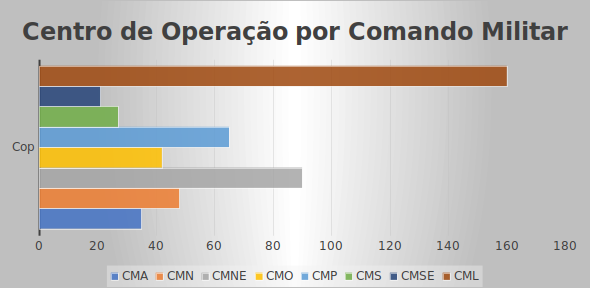
\includegraphics[width=1\textwidth]{Figuras/qtde2_cops.png}
        \caption{Gráfico de COps por Comandos Militar.}
        \label{figuraCops}
\end{figure}

% \hspace{1.5cm}
\textbf{Tabela \ref{QuantidadeAgentes}} É apresentado a distribuição de frequências do número de Agente numa amostra dos Comando Militar de Área do Exército Brasileiro. 

% Agentes
\begin{table}[H]
\centering
\begin{tabular}{|c | c| c|} 
 \multicolumn{3}{c}{Agente por Comando Militar}\\ \hline
  Comando Militar & freq  & percentagem \\ [0.5ex] 
 \hline
 Comando Militar da Amazônia (CMA) &  1224 & 4,88\\ 
 \hline
 Comando Militar do Norte (CMN) &  1496 & 5,97\\
 \hline
 Comando Militar do Nordeste (CMNE) &  4350 & 17,36\\
 \hline
 Comando Militar do Oeste (CMO) &  336 & 1,34\\
 \hline
 Comando Militar do Planalto (CMP) &  1026 & 4,09\\
 \hline
 Comando Militar do Sul (CMS) &  350 & 1,40\\
 \hline
 Comando Militar do Sudeste (CMSE) &  2196 & 8,76\\
 \hline
 Comando Militar do Leste (CML) &  14082 & 56,19\\ [1ex] 
 \hline
\end{tabular}
\caption{Quantidade de Agentes por Comando Militar de Área}
\label{QuantidadeAgentes}
\end{table}

% \hspace{1.5cm}
A representação gráfica da distribuição de frequência dos Agentes é dada pelo gráfico \ref{figuraAgentes}.
\begin{figure}[H]
        \centering
        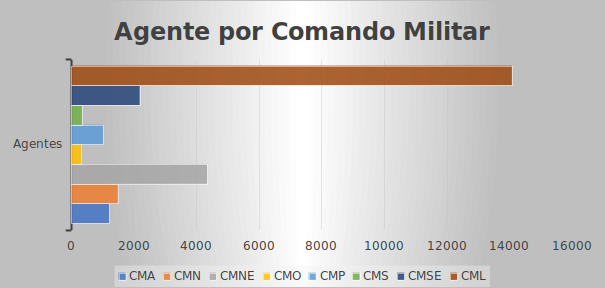
\includegraphics[width=1\textwidth]{Figuras/qtde_agentes.png}
        \caption{Gráfico de Agentes por Comandos Militar.}
        \label{figuraAgentes}
\end{figure}

% \hspace{1.5cm}
\textbf{Tabela \ref{QuantidadeIncidentes}} É apresentado a distribuição de frequências do número de Incidente numa amostra dos Comando Militar de Área do Exército Brasileiro. 
% Incidentes
\begin{table}[H]
\centering
\begin{tabular}{|c | c| c|} 
 \multicolumn{3}{c}{Incidente por Comando Militar}\\ \hline
  Comando Militar & freq   & percentagem \\ [0.5ex] 
 \hline
 Comando Militar da Amazônia (CMA) & 2280 & 21,80\\ 
 \hline
 Comando Militar do Norte (CMN) &  2301 & 22,00\\
 \hline
 Comando Militar do Nordeste (CMNE) &  3774 & 36,09\\
 \hline
 Comando Militar do Oeste (CMO) & 259 & 2,48\\
 \hline
 Comando Militar do Planalto (CMP) &  154 & 1,47\\
 \hline
 Comando Militar do Sul (CMS) &  203 & 1,94\\
 \hline
 Comando Militar do Sudeste (CMSE) &  79 & 0,76\\
 \hline
 Comando Militar do Leste (CML) &  1407 & 13,46\\ [1ex] 
 \hline
\end{tabular}
\caption{Quantidade de Incidentes por Comando Militar de Área}
\label{QuantidadeIncidentes}
\end{table}

% \hspace{1.5cm}
A representação gráfica da distribuição de frequência dos Incidentes é dada pelo gráfico \ref{figuraIncidentes}.
\begin{figure}[H]
        \centering
        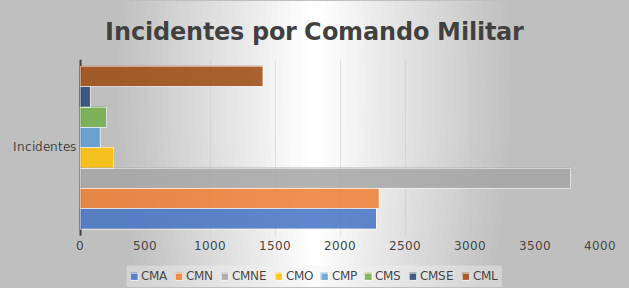
\includegraphics[width=1\textwidth]{Figuras/qtde_incidentes.png}
        \caption{Gráfico de Incidentes por Comandos Militar.}
        \label{figuraIncidentes}
\end{figure}

% \hspace{1.5cm}
\textbf{Tabela \ref{QuantidadeAcoes}} É apresentado a distribuição de frequências do número de Ação numa amostra dos Comando Militar de Área do Exército Brasileiro. 
% Ações
\begin{table}[H]
\centering
\begin{tabular}{|c | c| c|} 
 \multicolumn{3}{c}{Ação por Comando Militar}\\ \hline
  Comando Militar & freq   & percentagem \\ [0.5ex] 
 \hline
 Comando Militar da Amazônia (CMA) &  3193 & 22,22\\ 
 \hline
 Comando Militar do Norte (CMN) &  572 & 3,98\\
 \hline
 Comando Militar do Nordeste (CMNE) &  3009 & 20,94\\
 \hline
 Comando Militar do Oeste (CMO) &  3444 & 23,97\\
 \hline
 Comando Militar do Planalto (CMP) &  1031 & 7,18\\
 \hline
 Comando Militar do Sul (CMS) &  190 & 1,32\\
 \hline
 Comando Militar do Sudeste (CMSE) &  842 & 5,86\\
 \hline
 Comando Militar do Leste (CML) &  2087 & 14,53\\ [1ex] 
 \hline
\end{tabular}
\caption{Quantidade de Ações por Comando Militar de Área}
\label{QuantidadeAcoes}
\end{table}

% \hspace{1.5cm}
A representação gráfica da distribuição de frequência dos Ações é dada pelo gráfico \ref{figuraAcoes}.
\begin{figure}[H]
        \centering
        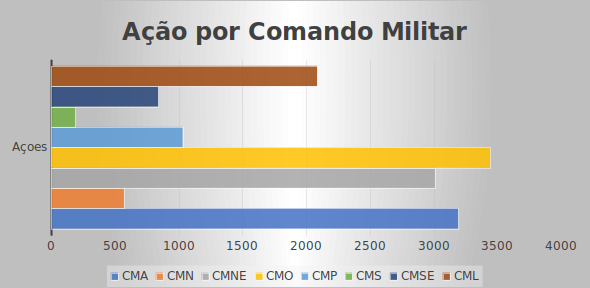
\includegraphics[width=1\textwidth]{Figuras/qtde_acoes.png}
        \caption{Gráfico de Ações por Comandos Militar.}
        \label{figuraAcoes}
\end{figure}

% \hspace{1.5cm}
\textbf{Tabela \ref{QuantidadeRelatos}} É apresentado a distribuição de frequências do número de Relato numa amostra dos Comando Militar de Área do Exército Brasileiro. 
% Relatos
\begin{table}[H]
\centering
\begin{tabular}{|c | c| c|} 
 \multicolumn{3}{c}{Relato por Comando Militar}\\ \hline
  Comando Militar & freq  & percentagem  \\ [0.5ex] 
 \hline
 Comando Militar da Amazônia (CMA) &  259 & 5,53\\ 
 \hline
 Comando Militar do Norte (CMN) &  371 & 7,93\\
 \hline
 Comando Militar do Nordeste (CMNE) &  1334 & 28,50\\
 \hline
 Comando Militar do Oeste (CMO) &  15 & 0,32\\
 \hline
 Comando Militar do Planalto (CMP) &  158 & 3,38\\
 \hline
 Comando Militar do Sul (CMS) &  611 & 13,06\\
 \hline
 Comando Militar do Sudeste (CMSE) &  1476 & 31,54\\
 \hline
 Comando Militar do Leste (CML) &  456 & 9,74\\ [1ex] 
 \hline
\end{tabular}
\caption{Quantidade de Relatos por Comando Militar de Área}
\label{QuantidadeRelatos}
\end{table}

% \hspace{1.5cm}
A representação gráfica da distribuição de frequência dos Relatos é dada pelo gráfico \ref{figuraRelatos}.
\begin{figure}[H]
        \centering
        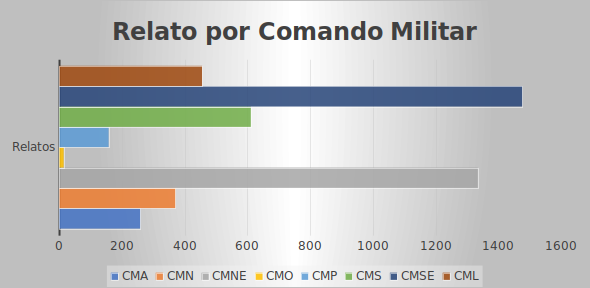
\includegraphics[width=1\textwidth]{Figuras/qtde_relatos.png}
        \caption{Gráfico de Relatos por Comandos Militar.}
        \label{figuraRelatos}
\end{figure}

%\hspace{1.5cm}
%\textbf{Tabela \ref{QuantidadeKmls}} É apresentado a distribuição de frequências do número de Kml numa amostra dos Comando Militar de Área do Exército Brasileiro. 
% Kmls
% \begin{table}[H]
% \centering
% \begin{tabular}{|c | c| c|} 
%  \multicolumn{3}{c}{Kml por Comando Militar}\\ \hline
%   Comando Militar & freq  & percentagem  \\ [0.5ex] 
%  \hline
%  Comando Militar da Amazônia (CMA) &  40 & 11,17\\ 
%  \hline
%  Comando Militar do Norte (CMN) &  21 & 5,87\\
%  \hline
%  Comando Militar do Nordeste (CMNE) &  92 & 25,70\\
%  \hline
%  Comando Militar do Oeste (CMO) &  18 & 5,03\\
%  \hline
%  Comando Militar do Planalto (CMP) &  40 & 11,17\\
%  \hline
%  Comando Militar do Sul (CMS) &  4 & 1,12\\
%  \hline
%  Comando Militar do Sudeste (CMSE) &  14 & 3,91\\
%  \hline
%  Comando Militar do Leste (CML) &  129 & 36,03\\ [1ex] 
%  \hline
% \end{tabular}
% \caption{Quantidade de Kmls por Comando Militar de Área}
% \label{QuantidadeKmls}
% \end{table}

%\hspace{1.5cm}
%A representação gráfica da distribuição de frequência dos Kmls é dada pelo gráfico \ref{figuraKmls}
% \begin{figure}[H]
%         \centering
%         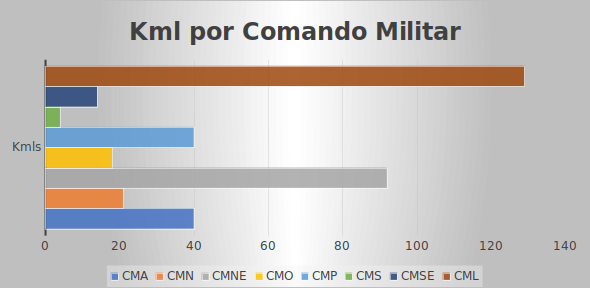
\includegraphics[width=1\textwidth]{Figuras/qtde_kmls.png}
%         \caption{Gráfico de Kmls por Comandos Militar.}
%         \label{figuraKmls}
% \end{figure}

% \hspace{1.5cm}
\textbf{Tabela \ref{QuantidadePois}} É apresentado a distribuição de frequências do número de Ponto de referência (POI) numa amostra dos Comando Militar de Área do Exército Brasileiro. 
% Pois
\begin{table}[H]
\centering
\begin{tabular}{|c | c| c|} 
 \multicolumn{3}{c}{Ponto de Interesse Operação por Comando Militar}\\ \hline
  Comando Militar & freq  & percentagem  \\ [0.5ex] 
 \hline
 Comando Militar da Amazônia (CMA) &  373 & \\ 
 \hline
 Comando Militar do Norte (CMN) &  61 & 3,44\\
 \hline
 Comando Militar do Nordeste (CMNE) &  357 & 20,16\\
 \hline
 Comando Militar do Oeste (CMO) &  14 & 0,79\\
 \hline
 Comando Militar do Planalto (CMP) &  55 & 3,11\\
 \hline
 Comando Militar do Sul (CMS) &  117 & 6,61\\
 \hline
 Comando Militar do Sudeste (CMSE) &  137 & 7,74\\
 \hline
 Comando Militar do Leste (CML) &  657 & 37,10\\ [1ex] 
 \hline
\end{tabular}
\caption{Quantidade de Ponto de interesse por Comando Militar de Área}
\label{QuantidadePois}
\end{table}

% \hspace{1.5cm}
A representação gráfica da distribuição de frequência dos COps é dada pelo gráfico \ref{figuraPois}
\begin{figure}[H]
        \centering
        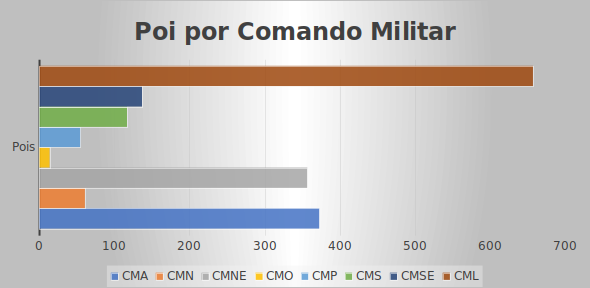
\includegraphics[width=1\textwidth]{Figuras/qtde_pois.png}
        \caption{Gráfico de Pontos de interesse por Comandos Militar.}
        \label{figuraPois}
\end{figure}

% \hspace{1.5cm}
Através do modelo de análise proposto, é possível verificar, tabela \ref{QuantidadeAgentes}. que no CML - Comando Militar do Leste, a utilização de agentes possui uma frequência superior aos demais comandos, devido as intervenções militares e as diversas atuações do comando na garantia da Lei e da Ordem no referido Estado. É importante destacar que na análise de ações por comando, tabela \ref{QuantidadeAcoes}, observa-se uma utilização substancial no CMO - Comando Militar do Oeste e CMA - Comando Militar da Amazônia, devido as queimadas no centro-oeste e no norte do país em 2019, além do crescente fluxo migratório na região do extremo norte, ocasionando portanto a maior utilização do Sistema Pacificador pelos referidos Comandos Militares. Observando os resultados das tabelas e gráficos percebemos que, através das frequências das variáveis por categoria, a utilização do Sistema de Comando e Controle pelos os Comandos Militares de Área demostra o crescimento da ferramenta Pacificador como reforço aos comandantes, nos diversos níveis, no controle dos elementos que compõem sua Força Tarefa durante um determinado Grande evento, Operações e atividade de Garantia da Lei e Ordem. 
 
